\chapter{操作系统接口}

操作系统的任务是让多个程序共享计算机,并且除了硬件已经支持的服务之外,还要提供更多有用的服务。
操作系统对底层的硬件进行管理和抽象,例如,一个字处理程序不需要关心它自己正在使用什么类型的磁盘。
它还在多个程序之间共享硬件,来让它们同时(或者看起来同时)运行。
最后,操作系统还提供可控的方式以允许程序进行交互,因此它们可以共享数据或者协同工作。

一个操作系统通过接口向用户称需提供服务。
设计一个好的接口被证明是非常困难的。
一方面,我们希望接口尽量简单和特化,因为这样可以更容易地正确实现它们。
另一方面,我们还希望向应用提供很多复杂的特性。
解决这种问题的方法是设计可以通过一些机制进行组合来提供复杂服务的简单接口。

这本书使用一个单独的操作系统作为具体的例子来展示操作系统的概念。
该操作系统,xv6,提供了Ken Thompson和Dennis Ritchie的Unix操作系统中引入的基本接口,同时模仿了Unix的内部设计。
Unix提供了一个特化的接口,但它们的机制结合得非常好,提供了惊人的通用性。
这个接口如此成功,以至于现代操作系统——BSD,Linux,Mac OS X,Solaris,甚至在小范围内,就连Microsoft Windows都有类Unix接口。
理解xv6是理解这些现代操作系统的一个好的开始。

如\autoref{f0-1}所示,xv6采用了\emph{内核(kernel)}的传统模式,内核是一个为运行中的程序提供服务的特殊程序。
每一个运行中的程序被称为一个\emph{进程(process)},它们都拥有包含指令、数据、栈的内存空间。
指令实现了程序的计算过程。
数据是计算操作时的变量。
栈用于组织程序的过程调用。

\begin{figure}[htbp]
    \centering
    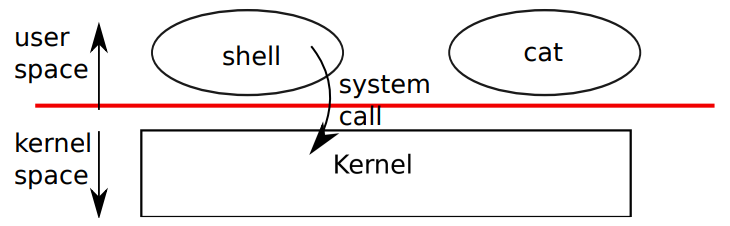
\includegraphics[width=0.8\textwidth]{../imgs/f0-1.png}
    \caption{一个内核和两个用户进程}
    \label{f0-1}
\end{figure}

当一个进程需要调用一个内核服务时,它会调用操作系统接口中的一个过程调用。
这样的过程被称为\emph{系统调用(system call)}。
系统调用会进入内核,然后内核执行服务并返回。
因此一个进程会在\emph{用户空间(user space)}和\emph{内核空间(kernel space)}中交替执行。

内核使用CPU的硬件保护机制来保证每个在用户空间执行的进程只能访问它自己的内存。
内核在执行时需要硬件特权来实现这些保护;而用户程序执行时没有特权。
当一个用户程序调用一个系统调用时,硬件会提高特权等级,然后开始执行内核中事先设置好的一个函数。

一个内核提供的系统调用的集合就是用户程序看到的接口。
xv6内核提供了Unix内核通常提供的服务和系统调用的一个子集。
\autoref{f0-2}列出了xv6的所有系统调用。

\begin{figure}[htbp]
    \centering
    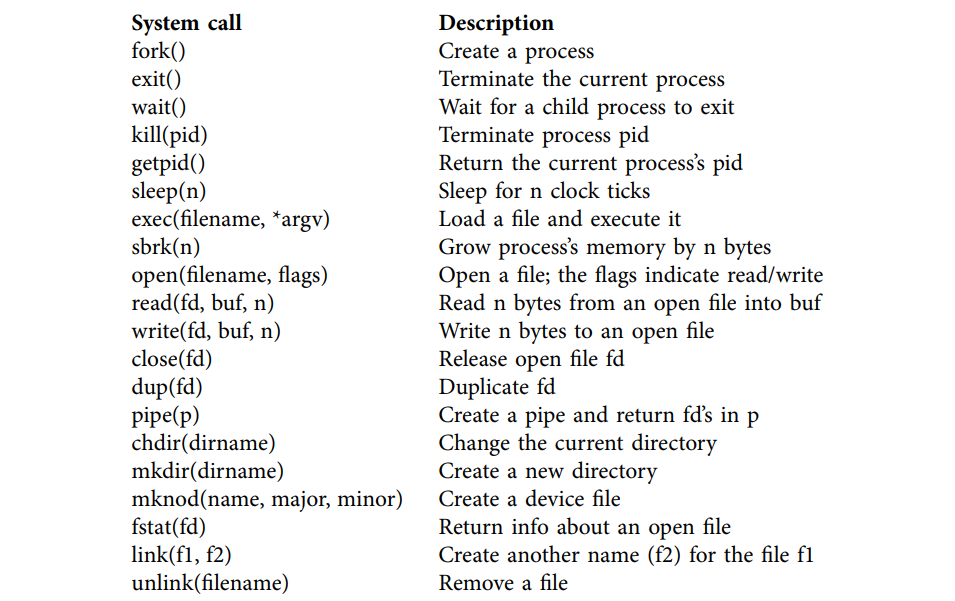
\includegraphics[width=0.8\textwidth]{../imgs/f0-2.png}
    \caption{xv6的系统调用}
    \label{f0-2}
\end{figure}

本章的剩余部分概述了xv6的服务——进程、内存、文件描述符、管道、文件系统——并且通过代码片段对它们进行说明,并讨论\emph{shell}(与传统的类Unix系统交互的主要用户接口)如何使用它们。
shell对系统调用的使用展示了它们的设计有多么精巧。

shell是一个读取用户的命令然后执行它们的普通程序。
它是一个用户程序,不是内核的一部分。
这一事实展示了系统调用接口的强大:shell并没有什么特殊的地方。
这也意味着shell可以很容易的替换;因此,现代Unix系统有很多shell可以选择,每一个都有自己的用户借口和脚本特性。
xv6的shell是Unix Bourne Shell的基础部分的一个简单实现。
它的实现可以在行(8550)找到。

\section*{处理器和内存}

一个xv6进程由用户空间内存(指令、数据、栈)和内核中私有的每个进程的状态组成。
xv6可以\emph{分时(time-share)}处理:它在一个等待执行的进程的集合中透明地切换可用的CPU。
当一个进程不在执行时,xv6会保存它的CPU寄存器,并在下一次执行这个进程时恢复它们。
内核为每个进程关联一个进程标识符,或者叫\texttt{pid}。

一个进程可能会使用\texttt{fork}系统调用创建一个新的进程。
\texttt{fork}会创建一个新的进程,称为\emph{子进程(child process)},它和调用者进程(称为\emph{父进程(parent process)})有完全相同的内存内容。
\texttt{fork}在父进程和子进程中都会返回。
在父进程中,\texttt{fork}会返回子进程的pid;而在子进程中它返回0。
例如,考虑下面的程序片段:

\begin{lstlisting}
    int pid = fork();
    if (pid > 0) {
        printf("parent: child=%d\n", pid);
        pid = wait();
        printf("child %d is done\n", pid);
    } else if (pid == 0) {
        printf("child: exiting\n");
        exit();
    } else {
        printf("fork error\n");
    }
\end{lstlisting}

\texttt{exit}系统调用会让调用者进程停止执行并释放资源,例如内存和打开的文件。
\texttt{wait}系统调用返回当前进程的一个退出的子进程的pid;如果调用者的子进程都还没有退出,那么\texttt{wait}会等待一个子进程退出。
在这个例子中,会输出:
\begin{blacklisting}
    parent: child=1234
    child: exiting
\end{blacklisting}    

也可能以其他顺序输出,取决于父进程还是子进程先到达\texttt{printf}调用。
当子进程退出后,父进程的\texttt{wait}会返回,然后父进程会打印出
\begin{blacklisting}
    parent: child 1234 is done
\end{blacklisting}

尽管子进程一开始有和父进程同样的内存内容,但父进程和子进程是在不同的内存和不同的寄存器中执行:修改其中一个的变量并不会影响另一个中同名的变量。
例如,当父进程中\texttt{wait}的返回值被存储到\texttt{pid}中时,并不会修改子进程中的\texttt{pid}变量。
子进程中的\texttt{pid}仍然是0。

\texttt{exec}系统调用会把调用者进程的内存替换为从文件系统的某个文件中加载的一个新的内存镜像。
这个文件必须有特定的格式,这个格式指定了文件中哪一部分存储指令、哪一部分是数据、从哪一条指令开始执行,等等。
xv6使用ELF格式,\autoref{ch02}中将会详细介绍这种格式。
当\texttt{exec}成功时,它并不会返回到调用者程序;而是开始执行从文件中加载的指令,执行的起点是ELF头中声明的入口点。
\texttt{exec}有两个参数:包含可执行程序的文件名,和一个字符串参数的数组。
例如:
\begin{lstlisting}
    char *argv[3];

    argv[0] = "echo";
    argv[1] = "hello";
    argv[2] = 0;
    exec("/bin/echo", argv);
    printf("exec error\n");
\end{lstlisting}

这个片段将调用者程序替换为\texttt{/bin/echo}程序的实例,并以\texttt{echo hello}作为参数列表。
大多数程序会忽略第一个参数,按照惯例它是程序的名称。

xv6 shell使用上面的调用来代替用户运行程序。shell的主要架构很简单,见\texttt{main}(8701)。
主循环使用\texttt{getcmd}读取用户的一行输入。
然后它调用\texttt{fork},创建一个shell进程的拷贝。
父进程调用\texttt{wait},而子进程运行读入的命令。
例如,如果用户向shell输入了“\texttt{echo hello}”,\texttt{runcmd}将会以“\texttt{echo hello}”为参数被调用。
\texttt{runcmd}(8606)运行实际的命令。
对于“\texttt{echo hello}”,它会调用\texttt{exec}(8626)。
如果\texttt{exec}成功,那么子进程会执行来自\texttt{echo}的指令而不是\texttt{runcmd}。
在某个时间点\texttt{echo}会调用\texttt{exit},这导致父进程从\texttt{main}(8701)中的\texttt{wait}返回。
你可能想知道为什么\texttt{fork}和\texttt{exec}不被合并成单个系统调用;我们稍后将会看到把创建进程和加载程序分离是一个聪明的设计。

xv6隐式分配大多数用户空间的内存:\texttt{fork}会为子进程分配内存来存储父进程内存的拷贝,\texttt{exec}会分配足够的内存来存储可执行文件。
一个进程如果在运行时需要更多的内存(可能是调用了\texttt{malloc}),可以调用\texttt{sbrk(n)}来把它的数据内存增大\texttt{n}个字节;\texttt{sbrk}返回新的内存的位置。

xv6不提供用户的概念、没有保护一个用户的文件不会被另一个用户修改的机制;用Unix术语来说就是,所有xv6进程都以root身份运行。

